\begin{frame}{Example with Dependent Inputs} % How does it look?
    \begin{align*}
    y(x_1, x_2) = 2x_1 + x_2^{2} + x_1 x_2, \qquad \rho = 0.8
  \end{align*}
  \begin{columns}
    \column{0.5\textwidth}
      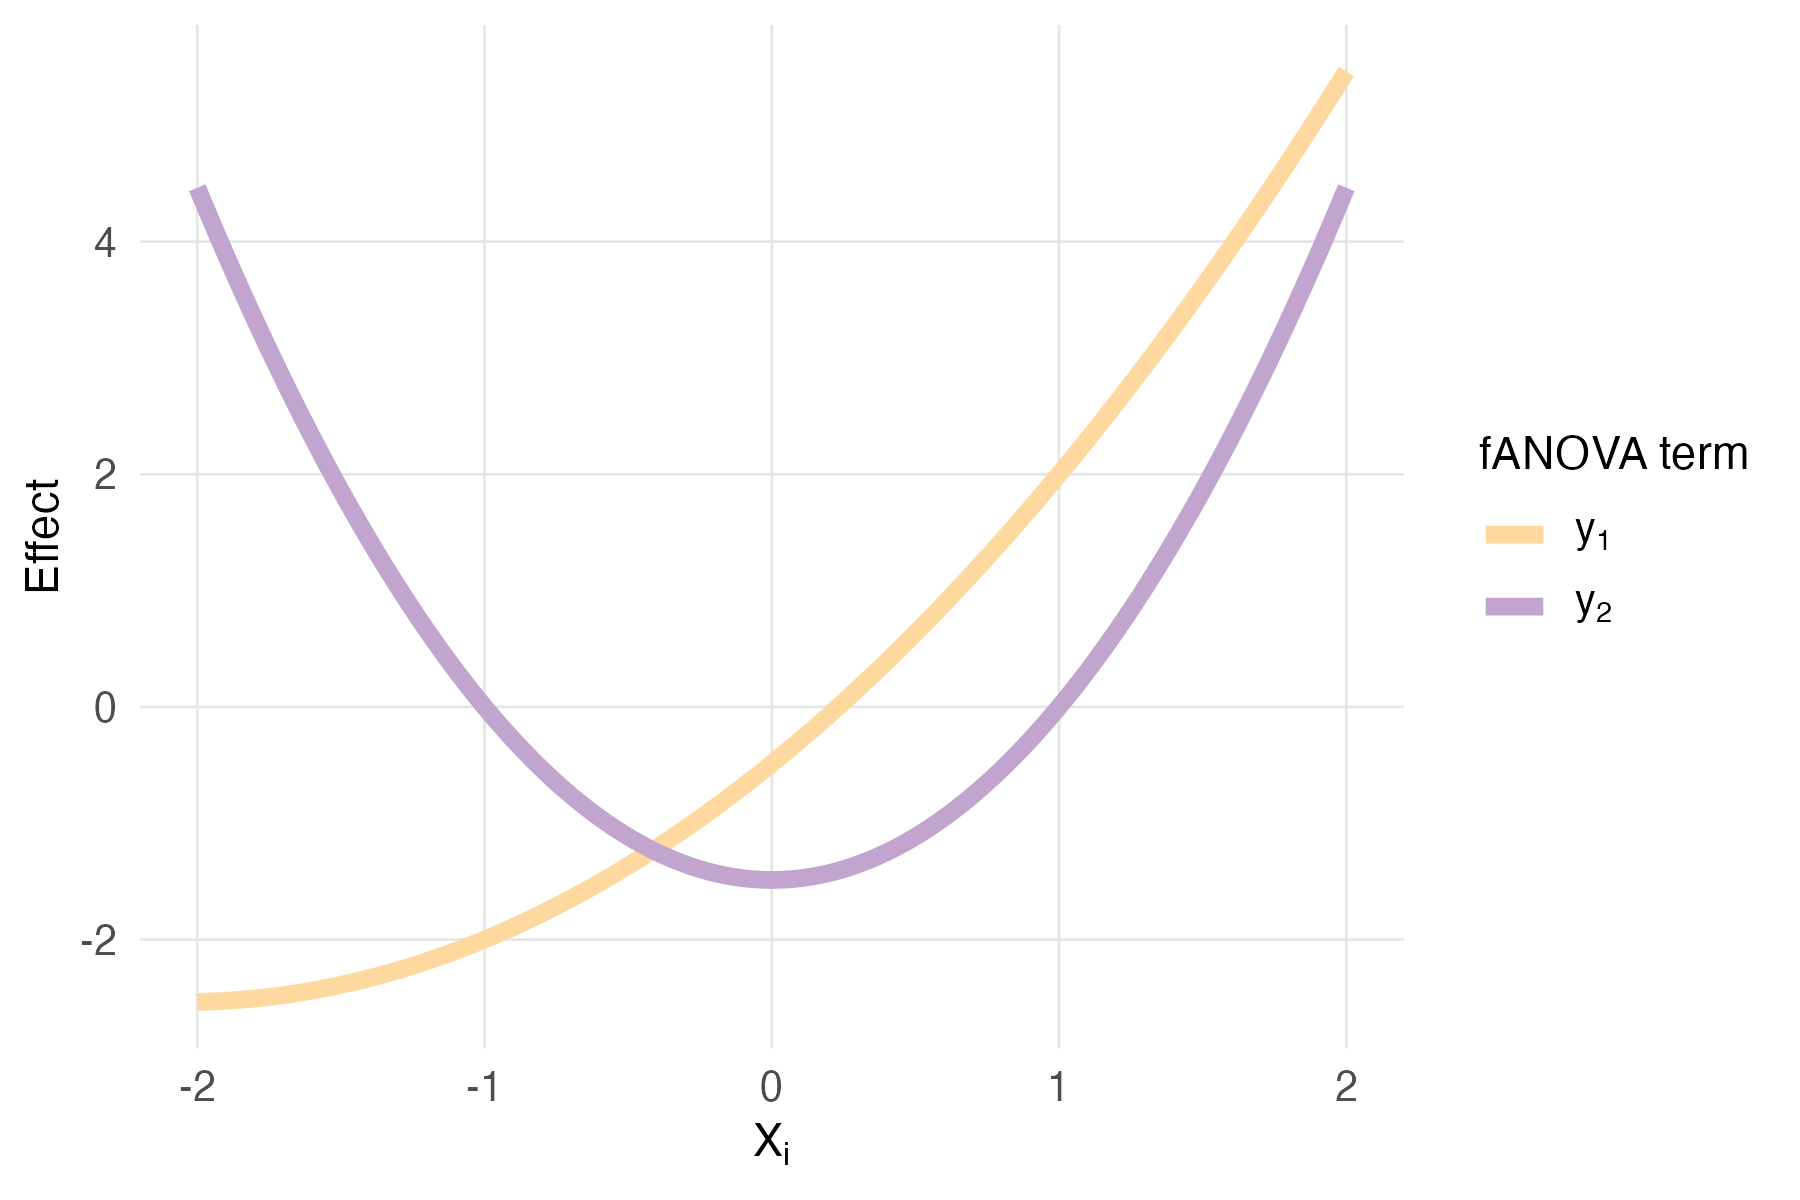
\includegraphics[width=\linewidth]{../images/experiment_section/gen_ex_1_a1p20_a2p00_a11p00_a22p10_a12p10_rhop08_main.png}
    \column{0.5\textwidth}
      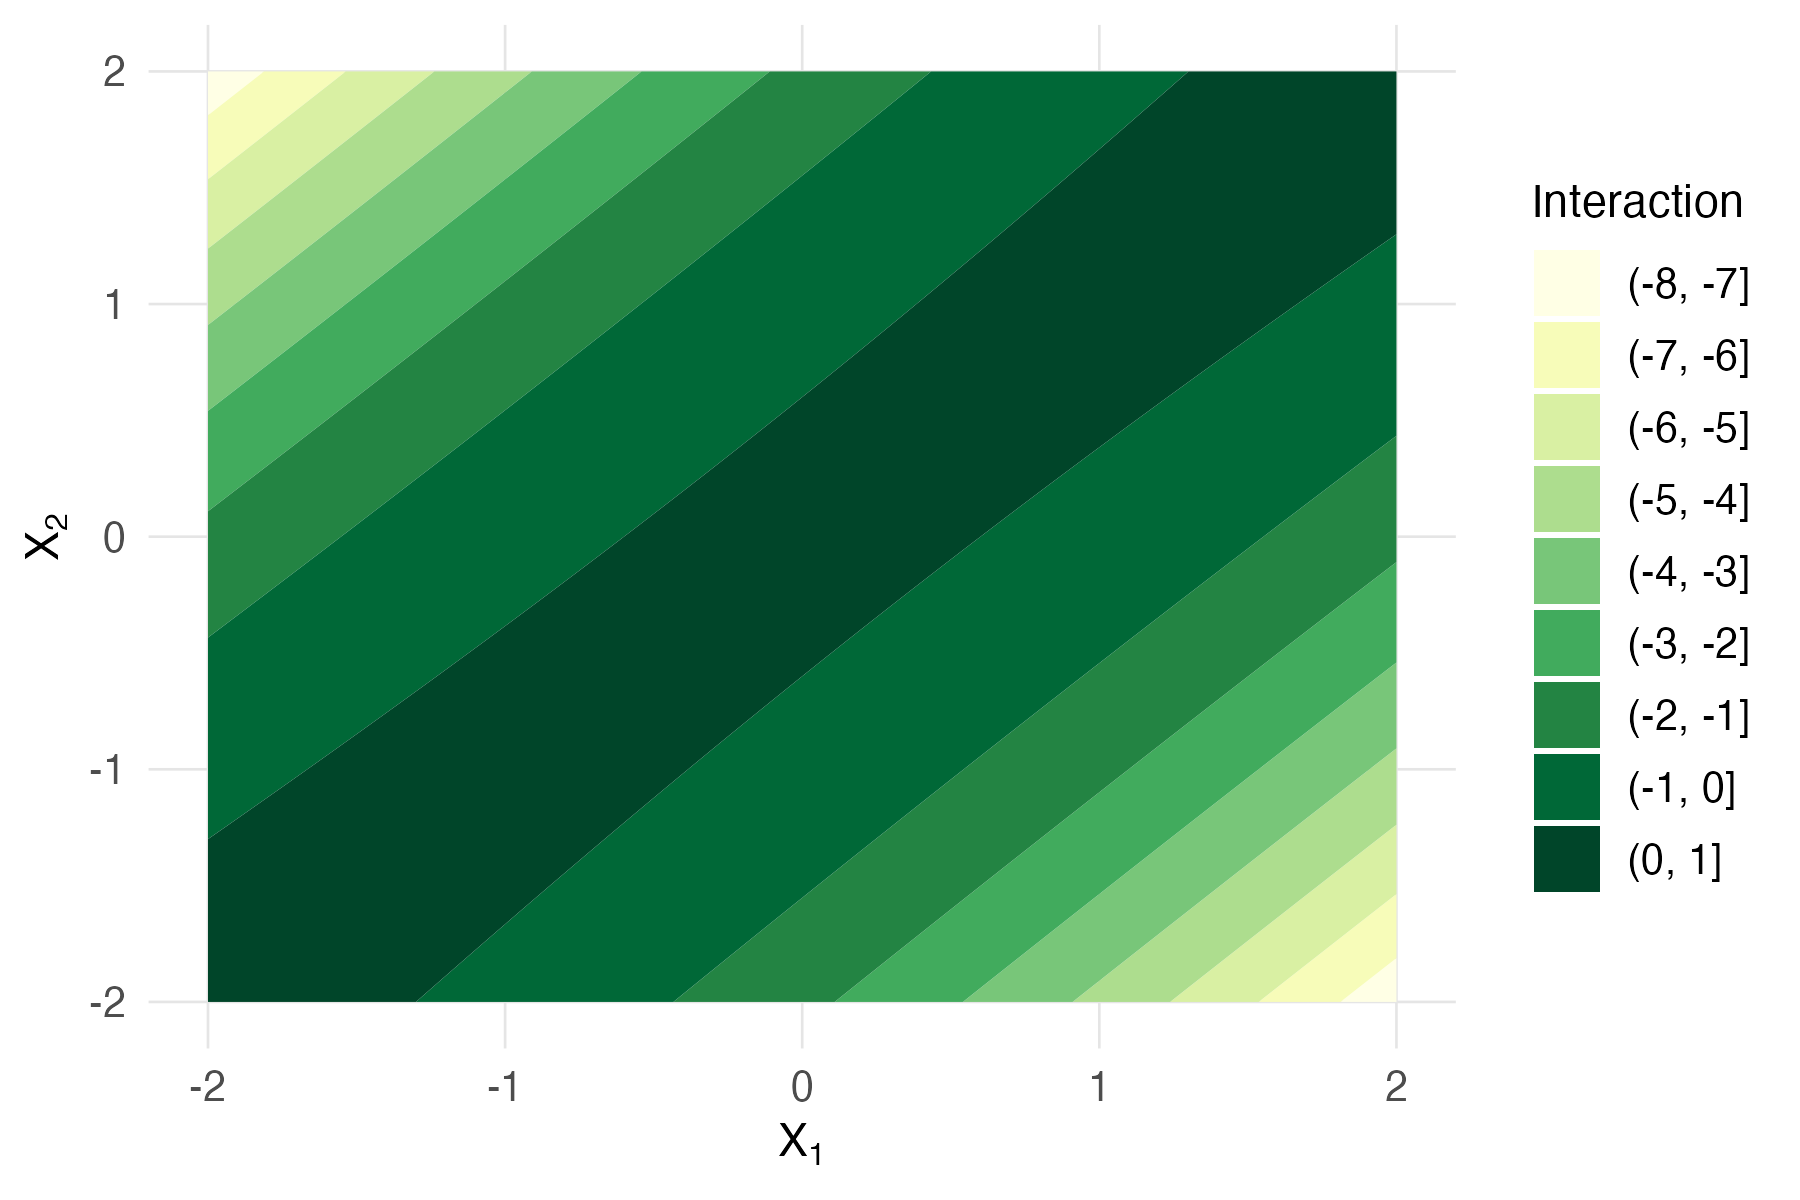
\includegraphics[width=\linewidth]{../images/experiment_section/gen_ex_1_a1p20_a2p00_a11p00_a22p10_a12p10_rhop08_interaction.png}
  \end{columns}
\end{frame}

%==================================================
% Slide 2 – Conditions (Weaker Annihilating Conditions)
%==================================================
\begin{frame}{Weaker Annihilating Conditions}
  \begin{block}{Weak Annihilating Conditions}
    \[
      \int_{\mathbb{R}} y_{u, G}(\boldsymbol{x}_u) f_{\boldsymbol{X}_u}(\boldsymbol{x}_u) d\nu (x_i) = 0 \quad \text{for} \quad i \in u \neq \emptyset.
    \]
  \end{block}
  \begin{itemize}
    \item Allows dependent input distributions
    \item Leads to hierarchical orthogonality
  \end{itemize}
    \[
  \mathbb{E}[y_{u, G}(\boldsymbol{X}_u)] := \int_{\mathbb{R}^N} y_{u, G}(\boldsymbol{x}_u) f_{\boldsymbol{X}}(\boldsymbol{x}) \, d\nu (\boldsymbol{x}) = 0.
  \]
  \[
  \mathbb{E}[y_{u, G}(\boldsymbol{X}_u)y_{v, G}(\boldsymbol{X}_v)] := \int_{\mathbb{R}^N} y_{u, G}(\boldsymbol{x}_u) y_{v, G}(\boldsymbol{x}_v) f_{\boldsymbol{X}}(\boldsymbol{x}) \, d\nu (\boldsymbol{x}) = 0.
  \]
\end{frame}


%==================================================
% Slide 4 – Construction
%==================================================
\begin{frame}{Component Definition (Coupled System)}
  \begin{align}
    y_{\emptyset,G} &= \int_{\mathbb{R}^N} y(\boldsymbol{x}) f_{\boldsymbol{X}}(\boldsymbol{x}) \, d \nu(\boldsymbol{x}) \\[3ex]
    y_{u,G}(\boldsymbol{X}_u) &= \int_{\mathbb{R}^{N - |u|}} y(\boldsymbol{X}_u, \boldsymbol{x}_{-u}) f_{-u}(\boldsymbol{x}_{-u}) \, d \nu(\boldsymbol{x}_{-u}) - \sum_{v \subsetneq u} y_{v,G}(\boldsymbol{X}_v) \notag \\
    &\quad - \sum_{\substack{\emptyset \ne v \subseteq \{1,\dots,N\} \\ v \cap u \ne \emptyset,\ v \not\subset u}} \int_{\mathbb{R}^{|v \cap -u|}} y_{v,G}(\boldsymbol{X}_{v \cap u}, \boldsymbol{x}_{v \cap -u}) f_{v \cap -u}(\boldsymbol{x}_{v \cap -u}) \, d \nu(\boldsymbol{x}_{v \cap -u}).
\end{align}
  \begin{itemize}
    \item All components solved simultaneously
    \item Depends on marginal densities and coupling terms
  \end{itemize}
\end{frame}

\begin{frame}
    \begin{itemize}
    \item $N = 3$
  \end{itemize}
    \begin{equation*}
    y_{\emptyset,G} = \int_{\mathbb{R}^3} y(\boldsymbol{x}) f_{\boldsymbol{X}}(\boldsymbol{x}) \, d \nu(\boldsymbol{x}) = \mathbb{E}[y(\boldsymbol{X})]
    \end{equation*}
    \begin{itemize}
      \item $u = \{1\}$
      \begin{itemize}
        \item $v \subsetneq u \rightarrow \emptyset$
        \item $(\emptyset \ne v \subseteq \{1,\dots,N\},\ v \cap u \ne \emptyset,\ v \not\subset u) \rightarrow \{1,2\}, \{1,2,3\}$
      \end{itemize}
    \end{itemize}

\end{frame}

%==================================================
% Slide 5 – Link Back to Example
%==================================================
\begin{frame}{How to Construct the Components}
    \begin{itemize}
        \item Coupled system $\rightarrow$ difficult to obtain analytical solutions
        \item Use alternative method via Fourier Polynomial (\cite{rahman2014})
        \item Building blocks: mutually orthogonal, zero-mean basis functions $\psi_{i, j}$, coefficients $c_{i, j}$
    \end{itemize}
\end{frame}

\begin{frame}{Basis Representation of a Polynomial}
    \begin{align*}
y(x_1,x_2) 
&= a_0 + a_1 x_1 + a_2 x_2 
   + a_{11} x_1^2 + a_{22} x_2^2 + a_{12} x_1 x_2 \\[0.5em]
&= c_0 
   + c_{1,1}\,\psi_{1,1}(x_1) 
   + c_{2,1}\,\psi_{2,1}(x_2) \\[0.5em]
&\quad
   + c_{1,2}\,\psi_{1,2}(x_1)
   + c_{2,2}\,\psi_{2,2}(x_2)
   + c_{12,11}\,\psi_{12,11}(x_1,x_2) \\[0.5em]
&= 
   \underbrace{c_0}_{y_0}
   + \underbrace{\big(c_{1,1}\,\psi_{1,1}(x_1) 
                     + c_{1,2}\,\psi_{1,2}(x_1)\big)}_{y_1(x_1)} \\[0.5em]
&\quad
   + \underbrace{\big(c_{2,1}\,\psi_{2,1}(x_2) 
                     + c_{2,2}\,\psi_{2,2}(x_2)\big)}_{y_2(x_2)} \\[0.5em]
&\quad
   + \underbrace{c_{12,11}\,\psi_{12,11}(x_1,x_2)}_{y_{12}(x_1,x_2)}.
\end{align*}
\end{frame}

\begin{frame}{Basis Functions proposed by Rahman (2014)\cite{rahman2014}}
    \begin{align*}
\psi_{\emptyset}(x_1,x_2) &= 1, \\[0.5em]
\psi_{1,1}(x_1) &= x_1, \\[0.5em]
\psi_{2,1}(x_2) &= x_2, \\[0.5em]
\psi_{1,2}(x_1) &= x_1^2 - 1, \\[0.5em]
\psi_{2,2}(x_2) &= x_2^2 - 1, \\[0.5em]
\psi_{12,11}(x_1,x_2) &= \frac{\rho (x_1^2 + x_2^2)}{1 + \rho^2} 
                         - x_1 x_2 
                         + \frac{\rho(\rho^2 - 1)}{1 + \rho^2},
\end{align*}
\end{frame}

\begin{frame}{Alternative Generalization of fANOVA, \cite{hooker2007}}
    \begin{align*}
\left\{ y_{u, G}(\boldsymbol{x}_u) \,\middle|\, u \subseteq d \right\}
= \arg\min_{\{g_u \in \mathcal{L}^2(\mathbb{R}^{|u|})\}} 
\int_{\mathbb{R}^N} \left( \sum_{u \subseteq d} g_u(\boldsymbol{x}_u) - y(\boldsymbol{x}) \right)^2 
f_{\boldsymbol{X}}(\boldsymbol{x}) \, d \nu (\boldsymbol{x}),
\label{eq:generalized_fanova_components_hooker}
\end{align*}
subject to hierarchical orthogonality conditions:
\begin{align*}
    \forall v \subseteq u,\ \forall g_v:\ 
    \int_{\mathbb{R}^N} y_u(\boldsymbol{x}_u) g_v(\boldsymbol{x}_v) 
    f_{\boldsymbol{X}}(\boldsymbol{x}) \, d \nu (\boldsymbol{x}) = 0.
\end{align*}
\end{frame}

\begin{frame}{Variance Decomposition, \cite{sobol1993sensitivity}}
    \[
    \mu := \mathbb{E}[y(\boldsymbol{X})] = y_{\emptyset,G}.
    \]
    \begin{align*}
\sigma^2 
&:= \mathbb{E}\left[ \left( y(\boldsymbol{X}) - \mu_G \right)^2 \right] \notag \\
&= \mathbb{E} \left[ \left( y_{\emptyset,G} + \sum_{u} y_{u,G}(\boldsymbol{X}_u) - y_{\emptyset,G} \right)^2 \right] \notag \\
&= \mathbb{E} \left[ \left( \sum_{u} y_{u,G}(\boldsymbol{X}_u) \right)^2 \right] \notag \\
&= \sum_{u} \mathbb{E} \left[ y_{u,G}^2(\boldsymbol{X}_u) \right]
+ \sum_{\substack{u \not\subseteq v,\, v \not\subseteq u}} 
\mathbb{E} \left[ y_{u,G}(\boldsymbol{X}_u) y_{v,G}(\boldsymbol{X}_v) \right],
\end{align*}
    
\end{frame}
